\documentclass[]{book}
\usepackage{lmodern}
\usepackage{amssymb,amsmath}
\usepackage{ifxetex,ifluatex}
\usepackage{fixltx2e} % provides \textsubscript
\ifnum 0\ifxetex 1\fi\ifluatex 1\fi=0 % if pdftex
  \usepackage[T1]{fontenc}
  \usepackage[utf8]{inputenc}
\else % if luatex or xelatex
  \ifxetex
    \usepackage{mathspec}
  \else
    \usepackage{fontspec}
  \fi
  \defaultfontfeatures{Ligatures=TeX,Scale=MatchLowercase}
\fi
% use upquote if available, for straight quotes in verbatim environments
\IfFileExists{upquote.sty}{\usepackage{upquote}}{}
% use microtype if available
\IfFileExists{microtype.sty}{%
\usepackage{microtype}
\UseMicrotypeSet[protrusion]{basicmath} % disable protrusion for tt fonts
}{}
\usepackage[margin=1in]{geometry}
\usepackage{hyperref}
\hypersetup{unicode=true,
            pdftitle={A Second Semester Statistics Course with R},
            pdfauthor={Mark Greenwood and Katherine Banner},
            pdfborder={0 0 0},
            breaklinks=true}
\urlstyle{same}  % don't use monospace font for urls
\usepackage{natbib}
\bibliographystyle{apalike}
\usepackage{color}
\usepackage{fancyvrb}
\newcommand{\VerbBar}{|}
\newcommand{\VERB}{\Verb[commandchars=\\\{\}]}
\DefineVerbatimEnvironment{Highlighting}{Verbatim}{commandchars=\\\{\}}
% Add ',fontsize=\small' for more characters per line
\usepackage{framed}
\definecolor{shadecolor}{RGB}{248,248,248}
\newenvironment{Shaded}{\begin{snugshade}}{\end{snugshade}}
\newcommand{\KeywordTok}[1]{\textcolor[rgb]{0.13,0.29,0.53}{\textbf{#1}}}
\newcommand{\DataTypeTok}[1]{\textcolor[rgb]{0.13,0.29,0.53}{#1}}
\newcommand{\DecValTok}[1]{\textcolor[rgb]{0.00,0.00,0.81}{#1}}
\newcommand{\BaseNTok}[1]{\textcolor[rgb]{0.00,0.00,0.81}{#1}}
\newcommand{\FloatTok}[1]{\textcolor[rgb]{0.00,0.00,0.81}{#1}}
\newcommand{\ConstantTok}[1]{\textcolor[rgb]{0.00,0.00,0.00}{#1}}
\newcommand{\CharTok}[1]{\textcolor[rgb]{0.31,0.60,0.02}{#1}}
\newcommand{\SpecialCharTok}[1]{\textcolor[rgb]{0.00,0.00,0.00}{#1}}
\newcommand{\StringTok}[1]{\textcolor[rgb]{0.31,0.60,0.02}{#1}}
\newcommand{\VerbatimStringTok}[1]{\textcolor[rgb]{0.31,0.60,0.02}{#1}}
\newcommand{\SpecialStringTok}[1]{\textcolor[rgb]{0.31,0.60,0.02}{#1}}
\newcommand{\ImportTok}[1]{#1}
\newcommand{\CommentTok}[1]{\textcolor[rgb]{0.56,0.35,0.01}{\textit{#1}}}
\newcommand{\DocumentationTok}[1]{\textcolor[rgb]{0.56,0.35,0.01}{\textbf{\textit{#1}}}}
\newcommand{\AnnotationTok}[1]{\textcolor[rgb]{0.56,0.35,0.01}{\textbf{\textit{#1}}}}
\newcommand{\CommentVarTok}[1]{\textcolor[rgb]{0.56,0.35,0.01}{\textbf{\textit{#1}}}}
\newcommand{\OtherTok}[1]{\textcolor[rgb]{0.56,0.35,0.01}{#1}}
\newcommand{\FunctionTok}[1]{\textcolor[rgb]{0.00,0.00,0.00}{#1}}
\newcommand{\VariableTok}[1]{\textcolor[rgb]{0.00,0.00,0.00}{#1}}
\newcommand{\ControlFlowTok}[1]{\textcolor[rgb]{0.13,0.29,0.53}{\textbf{#1}}}
\newcommand{\OperatorTok}[1]{\textcolor[rgb]{0.81,0.36,0.00}{\textbf{#1}}}
\newcommand{\BuiltInTok}[1]{#1}
\newcommand{\ExtensionTok}[1]{#1}
\newcommand{\PreprocessorTok}[1]{\textcolor[rgb]{0.56,0.35,0.01}{\textit{#1}}}
\newcommand{\AttributeTok}[1]{\textcolor[rgb]{0.77,0.63,0.00}{#1}}
\newcommand{\RegionMarkerTok}[1]{#1}
\newcommand{\InformationTok}[1]{\textcolor[rgb]{0.56,0.35,0.01}{\textbf{\textit{#1}}}}
\newcommand{\WarningTok}[1]{\textcolor[rgb]{0.56,0.35,0.01}{\textbf{\textit{#1}}}}
\newcommand{\AlertTok}[1]{\textcolor[rgb]{0.94,0.16,0.16}{#1}}
\newcommand{\ErrorTok}[1]{\textcolor[rgb]{0.64,0.00,0.00}{\textbf{#1}}}
\newcommand{\NormalTok}[1]{#1}
\usepackage{longtable,booktabs}
\usepackage{graphicx,grffile}
\makeatletter
\def\maxwidth{\ifdim\Gin@nat@width>\linewidth\linewidth\else\Gin@nat@width\fi}
\def\maxheight{\ifdim\Gin@nat@height>\textheight\textheight\else\Gin@nat@height\fi}
\makeatother
% Scale images if necessary, so that they will not overflow the page
% margins by default, and it is still possible to overwrite the defaults
% using explicit options in \includegraphics[width, height, ...]{}
\setkeys{Gin}{width=\maxwidth,height=\maxheight,keepaspectratio}
\IfFileExists{parskip.sty}{%
\usepackage{parskip}
}{% else
\setlength{\parindent}{0pt}
\setlength{\parskip}{6pt plus 2pt minus 1pt}
}
\setlength{\emergencystretch}{3em}  % prevent overfull lines
\providecommand{\tightlist}{%
  \setlength{\itemsep}{0pt}\setlength{\parskip}{0pt}}
\setcounter{secnumdepth}{5}
% Redefines (sub)paragraphs to behave more like sections
\ifx\paragraph\undefined\else
\let\oldparagraph\paragraph
\renewcommand{\paragraph}[1]{\oldparagraph{#1}\mbox{}}
\fi
\ifx\subparagraph\undefined\else
\let\oldsubparagraph\subparagraph
\renewcommand{\subparagraph}[1]{\oldsubparagraph{#1}\mbox{}}
\fi

%%% Use protect on footnotes to avoid problems with footnotes in titles
\let\rmarkdownfootnote\footnote%
\def\footnote{\protect\rmarkdownfootnote}

%%% Change title format to be more compact
\usepackage{titling}

% Create subtitle command for use in maketitle
\newcommand{\subtitle}[1]{
  \posttitle{
    \begin{center}\large#1\end{center}
    }
}

\setlength{\droptitle}{-2em}
  \title{A Second Semester Statistics Course with R}
  \pretitle{\vspace{\droptitle}\centering\huge}
  \posttitle{\par}
  \author{Mark Greenwood and Katherine Banner}
  \preauthor{\centering\large\emph}
  \postauthor{\par}
  \predate{\centering\large\emph}
  \postdate{\par}
  \date{2017-07-21}

\usepackage{booktabs}
\usepackage[nottoc,numbib]{tocbibind}
\usepackage{amsmath}
\usepackage{color}
\usepackage{amsbsy}
\usepackage[normalem]{ulem}
\usepackage{cancel}
\usepackage[svgnames]{xcolor}
\usepackage{float}

\definecolor{purple}{RGB}{76,0,153}

% % make code-output smaller
% \DefineVerbatimEnvironment{Highlighting}{Verbatim}{fontsize=\tiny,commandchars=\\\{\}}
% 

% make console-output smaller:
  \makeatletter
\def\verbatim{\small\@verbatim \frenchspacing\@vobeyspaces \@xverbatim}
\makeatother


%\setlength{\parskip}{0pt}


\setlength{\OuterFrameSep}{-4pt}
\makeatletter
\def\preto{\@verbatim}{\topsep=-10pt \partopsep=-10pt }
\makeatother

\usepackage{amsthm}
\newtheorem{theorem}{Theorem}[chapter]
\newtheorem{lemma}{Lemma}[chapter]
\theoremstyle{definition}
\newtheorem{definition}{Definition}[chapter]
\newtheorem{corollary}{Corollary}[chapter]
\newtheorem{proposition}{Proposition}[chapter]
\theoremstyle{definition}
\newtheorem{example}{Example}[chapter]
\theoremstyle{remark}
\newtheorem*{remark}{Remark}
\begin{document}
\maketitle

{
\setcounter{tocdepth}{1}
\tableofcontents
}
\chapter*{Acknowledgments}\label{acknowledgments}
\addcontentsline{toc}{chapter}{Acknowledgments}

We would like to thank all the students and instructors who have
provided input in the development of the current version of STAT 217 and
that have impacted the choice of topics and how we try to teach them.
Dr.~Robison-Cox initially developed this course using R and much of this
work retains his initial ideas. Many years of teaching these topics and
helping researchers use these topics has helped to refine how they are
presented here. Observing students years after the course has also
helped to refine what we try to teach in the course, trying to prepare
these students for the next levels of statistics courses that they might
encounter and the next class where they might need or want to use
statistics.

I (Greenwood) have intentionally taken a first person perspective at
times to be able to include stories from some of those interactions to
try to help you avoid some of their pitfalls in your current or future
usage of statistics. I would like to thank my wife, Teresa Greenwood,
for allowing me the time and support to work on this. I would also like
to acknowledge Dr.~Gordon Bril (Luther College) who introduced me to
statistics while I was an undergraduate and Dr.~Snehalata Huzurbazar
(University of Wyoming) that guided me to completing my Master's and
Ph.D.~in Statistics and still serves as a valued mentor and friend to
me.

The development of this text was initially supported with funding from
Montana State University's Instructional Innovation Grant Program with a
grant titled Towards more active learning in STAT 217. This book was
born with the goal of having a targeted presentation of topics that we
cover (and few that we don't) that minimizes cost to students and
incorporates the statistical software R from day one and every day after
that. The software is a free, open-source platform and so is dynamically
changing over time. This has necessitated frequent revisions of the
text.

This is Version 3.01 of the book. It fixes a problem created with the
digital links in the book that occurred during Spring 2017. Version 3.0
of the book, prepared for Fall 2016, involved edits, a couple of
partially new sections, and updated R code along with a new format for
how the R code is displayed to more easily distinguish it from other
text. Each revision has involved a similar amount of change with Version
2.0 published in January 2015 and Version 1.0 in January 2014 after
using draft chapters that were initially developed during Fall 2013.

We have made every attempt to keep costs as low as possible by making it
possible for most pages to be printed in black and white. The text (in
full color and with dynamic links) is also available as a free digital
download from Montana State University's ScholarWorks repository at
\url{https://scholarworks.montana.edu/xmlui/handle/1/2999}.

Enjoy your journey from introductory to intermediate statistics!

This work is licensed under the Creative Commons
Attribution-NonCommercial-NoDerivatives 4.0 International License. To
view a copy of this license, visit
\url{http://creativecommons.org/licenses/by-nc-nd/4.0/} or send a letter
to Creative Commons, 444 Castro Street, Suite 900, Mountain View,
California, 94041, USA.

\chapter{Chi-square tests}\label{chapter5}

\section{Situation, contingency tables, and plots}\label{section5-1}

In this chapter, the focus shifts briefly from analyzing quantitative
response variables to methods for handling categorical response
variables. This is important because in some situations it is not
possible to measure the response variable quantitatively. For example,
we will analyze the results from a clinical trial where the results for
the subjects were measured as one of three categories: \emph{no
improvement}, \emph{some improvement}, and \emph{marked improvement}.
While that type of response could be treated as numerical, coded
possibly as 1, 2, and 3, it would be difficult to assume that the
responses such as those follow a normal distribution since they are
\textbf{\emph{discrete}} (not continuous, measured at whole number
values only) and, more importantly, the difference between \emph{no
improvement} and \emph{some improvement} is not necessarily the same as
the difference between \emph{some} and \emph{marked improvement}. If it
is treated numerically, then the differences are assumed to be the same
unless a different coding scheme is used (say 1, 2, and 5). It is better
to treat these types of responses as being in one of the three
categories and use statistical methods that don't make unreasonable
assumptions about what the numerical coding might mean. The study being
performed here involved subjects randomly assigned to either a treatment
or a placebo (control) group and we want to address research questions
similar to those considered in Chapters \ref{chapter2} and
\ref{chapter3} -- assessing differences among two or more groups. With
quantitative responses, the differences in the distributions are
parameterized via the means of the groups and we used 2-sample mean or
ANOVA hypotheses and tests. With categorical responses, the focus is on
the probabilities of getting responses in each category and whether they
differ among the groups.

We start with some useful summary techniques, both numerical and
graphical, applied to some examples of studies these methods can be used
to analyze. Graphical techniques provide opportunities for assessing
specific patterns in variables, relationships between variables, and for
generally understanding the responses obtained. There are many different
types of plots and each can enhance certain features of data. We will
start with a ``fun'' display, called a tableplot, to help us understand
some aspects of the results from a double-blind randomized clinical
trial investigating a treatment for rheumatoid arthritis that has the
categorical response variable introduced previously. These data are
available in the \texttt{Arthritis} data set available in the
\texttt{vcd} package \citep{R-vcd}. There were \(n=84\) subjects, with
some demographic information recorded along with the \texttt{Treatment}
status (\emph{Treated}, \emph{Placebo}) and whether the patients'
arthritis symptoms \texttt{Improved} (with levels of \emph{None},
\emph{Some}, and \emph{Marked}).

The \texttt{tableplot} function from the \texttt{tabplot} package
\citep{R-tabplot} displays bars for each response in a row\footnote{In
  larger data sets, multiple subjects are displayed in each row as
  proportions of the rows in each category.} based on the category of
responses or as a bar with the height corresponding the value of
quantitative variables. It also plots a red cell if the observations
were missing on a particular variable. The plot can be obtained simply
as \texttt{tableplot(DATASETNAME)}. But when using \texttt{tableplot},
we may not want to display everything in the data.frame and often just
select some of the variables. We use \texttt{Treatment},
\texttt{Improved}, \texttt{Sex}, and \texttt{Age} in the
\texttt{select=...} option with a \texttt{c()} and commas between the
names of the variables we want to display. The first one in the list is
also the one that the data are sorted based on.



\begin{Shaded}
\begin{Highlighting}[]
\KeywordTok{require}\NormalTok{(vcd)}
\KeywordTok{data}\NormalTok{(Arthritis) }\CommentTok{#Double-blind clinical trial with treatment and control groups}
\CommentTok{#Homogeneity example}
\KeywordTok{require}\NormalTok{(tabplot)}
\KeywordTok{tableplot}\NormalTok{(Arthritis,}\DataTypeTok{select=}\KeywordTok{c}\NormalTok{(Treatment,Improved,Sex,Age))}
\end{Highlighting}
\end{Shaded}

\begin{figure}
\centering
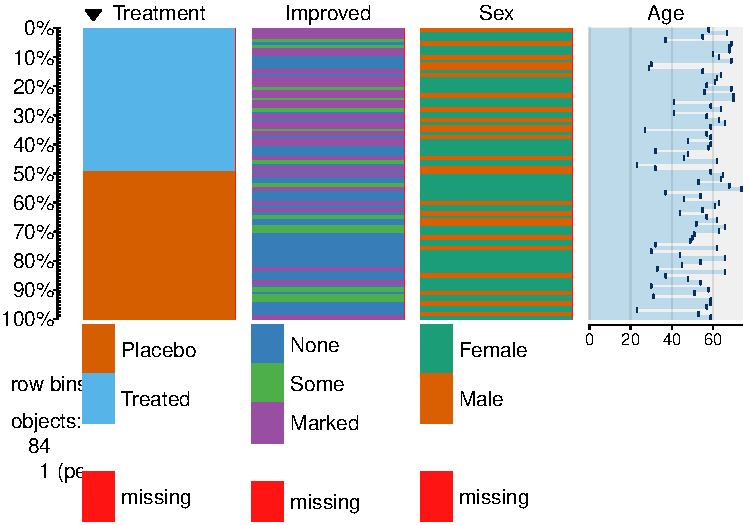
\includegraphics{05-chiSquaredTests_test_files/figure-latex/Figure5-1-1.pdf}
\caption{\label{fig:Figure5-1}Table plot of the arthritis data set.}
\end{figure}

The first thing we can gather from Figure \ref{fig:Figure5-1} is that
there are no red cells so there were no missing observations in the data
set. Missing observations regularly arise in real studies when
observations are not obtained for many different reasons and it is
always good to check for missing data issues -- this plot provides a
quick visual method for doing that check. Primarily we are interested in
whether the treatment led to a different pattern (or rates) of
improvement responses. There seems to be more purple (\emph{Marked})
improvement responses in the treatment group and more blue (\emph{None})
responses in the placebo group. This sort of plot also helps us to
simultaneously consider the role of other variables in the observed
responses. You can see the sex of each subject in the vertical panel for
\texttt{Sex} and it seems that there is a relatively reasonable mix of
males and females in the treatment/placebo groups. Quantitative
variables are also displayed with horizontal bars corresponding to the
responses. From the panel for \texttt{Age}, we can see that the ages of
subjects ranged from the 20s to 70s and that there is no clear
difference in the ages between the treated and placebo groups. If, for
example, all the male subjects had ended up being randomized into the
treatment group, then we might have worried about whether sex and
treatment were confounded and whether any differences in the responses
might be due to sex instead of the treatment. The random assignment of
treatment/placebo to the subjects appears to have been successful here
with the ages and sexes appearing to be well-mixed among the two
treatment groups. The main benefit of this sort of plot is the ability
to visualize more than two categorical variables simultaneously. But now
we want to focus more directly on the researchers' main question -- does
the treatment lead to different improvement outcomes than the placebo?

To directly assess the effects of the treatment, we want to display just
the two variables of interest. \textbf{\emph{Stacked bar charts}}
provide a method of displaying the response patterns (in
\texttt{Improved}) across the levels of a predictor
variable(\texttt{Treatment}) by displaying a bar for each predictor
variable level and the proportions of responses in each category of the
response in each of those groups. If the placebo is as effective as the
treatment, then we would expect similar proportions of responses in each
improvement category. A difference in the effectiveness would manifest
in different proportions in the different improvement categories between
\emph{Treated} and \emph{Placebo}. To get information in this direction,
we start with obtaining the counts in each combination of categories
using the \texttt{tally} function to generate contingency tables.
\textbf{\emph{Contingency tables}} with \textbf{\emph{R}} rows and
\textbf{\emph{C}} columns (called \textbf{\emph{R by C tables}})
summarize the counts of observations in each combination of the
explanatory and response variables. In these data, there are \(R=2\)
rows and \(C=3\) columns making a \(2\times 3\) table -- note that you
do not count the row and column for the ``Totals'' in defining the size
of the table. In the table, there seems to be many more \emph{Marked}
improvement responses (21 vs 7) and fewer \emph{None} responses (13 vs
29) in the treated group compared to the placebo group.

\begin{Shaded}
\begin{Highlighting}[]
\KeywordTok{require}\NormalTok{(mosaic)}
\KeywordTok{tally}\NormalTok{(}\OperatorTok{~}\NormalTok{Treatment}\OperatorTok{+}\NormalTok{Improved, }\DataTypeTok{data=}\NormalTok{Arthritis, }\DataTypeTok{margins=}\NormalTok{T)}
\end{Highlighting}
\end{Shaded}

\begin{verbatim}
##          Improved
## Treatment None Some Marked Total
##   Placebo   29    7      7    43
##   Treated   13    7     21    41
##   Total     42   14     28    84
\end{verbatim}

Using the \texttt{tally} function with \texttt{\textasciitilde{}x+y}
provides a contingency table with the \texttt{x} variable on the rows
and the \texttt{y} variable on the columns, with \texttt{margins=T} as
an option so we can obtain the totals along the rows, columns, and table
total of \(N=84\). In general, contingency tables contain the counts
\(n_{rc}\) in the \(r^{th}\) row and \(c^{th}\) column where
\(r=1,\ldots,R\) and \(c=1,\ldots,C\). We can also define the
\textbf{\emph{row totals}} as the sum across row \(r\) as

\[\mathbf{n_{r\bullet}}=\Sigma^C_{c=1}n_{rc},\] the \textbf{\emph{column
totals}} as the sum across column \(c\) as

\[\mathbf{n_{\bullet c}}=\Sigma^R_{r=1}n_{rc},\]

and the \textbf{\emph{table total}} as

\[\mathbf{N}=\Sigma^R_{r=1}\mathbf{n_{r\bullet}} = \Sigma^C_{c=1}\mathbf{n_{\bullet c}}
= \Sigma^R_{r=1}\Sigma^C_{c=1}\mathbf{n_{rc}}.\]

We'll need these quantities to do some calculations in a bit. A generic
contingency table with added row, column, and table totals just like the
previous result from the \texttt{tally} function is provided in Table
\ref{tab:Table5-1}.



\begin{table}

\caption{\label{tab:Table5-1}General notation for counts in an R by C contingency table.}
\centering
\begin{tabular}[t]{l|l|l|l|l|l|l}
\hline
 & **Response Level 1** & Response Level 2 & Response Level 3 & ... & Response Level C & Totals\\
\hline
$\textbf{Group 1}$ & $n_{11}$ & $n_{12}$ & $n_{13}$ & $\ldots$ & $n_{1C}$ & $\mathbf{n_{1\bullet}}$\\
\hline
$\textbf{Group 2}$ & $n_{21}$ & $n_{22}$ & $n_{23}$ & $\ldots$ & $n_{2C}$ & $\mathbf{n_{2\bullet}}$\\
\hline
$\mathbf{\ldots}$ & $\ldots$ & $\ldots$ & $\ldots$ & $\ldots$ & $\ldots$ & $\mathbf{\ldots}$\\
\hline
$\textbf{Group R}$ & $n_{R1}$ & $n_{R2}$ & $n_{R3}$ & $\ldots$ & $n_{RC}$ & $\mathbf{n_{R\bullet}}$\\
\hline
$\textbf{Totals}$ & $\mathbf{n_{\bullet 1}}$ & $\mathbf{n_{\bullet 2}}$ & $\mathbf{n_{\bullet 3}}$ & $\mathbf{\ldots}$ & $\mathbf{n_{\bullet C}}$ & $\mathbf{N}$\\
\hline
\end{tabular}
\end{table}

Comparing counts from the contingency table is useful, but comparing
proportions in each category is better, especially when the sample sizes
in the levels of the explanatory variable differ. Switching the formula
used in the \texttt{tally} function formula to
\texttt{\textasciitilde{}\ y\ \textbar{}\ x} and adding the
\texttt{format="proportion"} option provides the proportions in the
response categories conditional on the category of the predictor (these
are called \textbf{\emph{conditional proportions}} or the
\textbf{\emph{conditional distribution}} of, here, \emph{Improved} on
\emph{Treatment})\footnote{The vertical line, ``\texttt{\textbar{}}'',
  in \texttt{\textasciitilde{}\ y\textbar{}x} is available on most
  keyboards on the same key as ``". It is the mathematical symbol that
  means''conditional on" whatever follows.}. Note that they sum to 1.0
in each level of x, \emph{placebo} or \emph{treated}: See
\ref{tab:Table5-2}



\begin{longtable}[]{@{}ccccccc@{}}
\caption{\label{tab:Table5-2} My table caption}\tabularnewline
\toprule
\begin{minipage}[b]{0.06\columnwidth}\centering\strut
~\strut
\end{minipage} & \begin{minipage}[b]{0.14\columnwidth}\centering\strut
\textbf{Response\\
Level 1}\strut
\end{minipage} & \begin{minipage}[b]{0.14\columnwidth}\centering\strut
\textbf{Response\\
Level 2}\strut
\end{minipage} & \begin{minipage}[b]{0.14\columnwidth}\centering\strut
\textbf{Response\\
Level 3}\strut
\end{minipage} & \begin{minipage}[b]{0.05\columnwidth}\centering\strut
\textbf{\ldots{}}\strut
\end{minipage} & \begin{minipage}[b]{0.14\columnwidth}\centering\strut
\textbf{Response\\
Level C}\strut
\end{minipage} & \begin{minipage}[b]{0.14\columnwidth}\centering\strut
\textbf{Totals}\strut
\end{minipage}\tabularnewline
\midrule
\endfirsthead
\toprule
\begin{minipage}[b]{0.06\columnwidth}\centering\strut
~\strut
\end{minipage} & \begin{minipage}[b]{0.14\columnwidth}\centering\strut
\textbf{Response\\
Level 1}\strut
\end{minipage} & \begin{minipage}[b]{0.14\columnwidth}\centering\strut
\textbf{Response\\
Level 2}\strut
\end{minipage} & \begin{minipage}[b]{0.14\columnwidth}\centering\strut
\textbf{Response\\
Level 3}\strut
\end{minipage} & \begin{minipage}[b]{0.05\columnwidth}\centering\strut
\textbf{\ldots{}}\strut
\end{minipage} & \begin{minipage}[b]{0.14\columnwidth}\centering\strut
\textbf{Response\\
Level C}\strut
\end{minipage} & \begin{minipage}[b]{0.14\columnwidth}\centering\strut
\textbf{Totals}\strut
\end{minipage}\tabularnewline
\midrule
\endhead
\begin{minipage}[t]{0.06\columnwidth}\centering\strut
\textbf{Group 1}\strut
\end{minipage} & \begin{minipage}[t]{0.14\columnwidth}\centering\strut
\(n_{11}\)\strut
\end{minipage} & \begin{minipage}[t]{0.14\columnwidth}\centering\strut
\(n_{12}\)\strut
\end{minipage} & \begin{minipage}[t]{0.14\columnwidth}\centering\strut
\(n_{13}\)\strut
\end{minipage} & \begin{minipage}[t]{0.05\columnwidth}\centering\strut
\ldots{}\strut
\end{minipage} & \begin{minipage}[t]{0.14\columnwidth}\centering\strut
\(n_{15}\)\strut
\end{minipage} & \begin{minipage}[t]{0.14\columnwidth}\centering\strut
\(n_{11}\)\strut
\end{minipage}\tabularnewline
\begin{minipage}[t]{0.06\columnwidth}\centering\strut
\textbf{Group 2}\strut
\end{minipage} & \begin{minipage}[t]{0.14\columnwidth}\centering\strut
\(n_{21}\)\strut
\end{minipage} & \begin{minipage}[t]{0.14\columnwidth}\centering\strut
\(n_{22}\)\strut
\end{minipage} & \begin{minipage}[t]{0.14\columnwidth}\centering\strut
\(n_{23}\)\strut
\end{minipage} & \begin{minipage}[t]{0.05\columnwidth}\centering\strut
\ldots{}\strut
\end{minipage} & \begin{minipage}[t]{0.14\columnwidth}\centering\strut
\(n_{25}\)\strut
\end{minipage} & \begin{minipage}[t]{0.14\columnwidth}\centering\strut
\(n_{21}\)\strut
\end{minipage}\tabularnewline
\begin{minipage}[t]{0.06\columnwidth}\centering\strut
\textbf{\ldots{}}\strut
\end{minipage} & \begin{minipage}[t]{0.14\columnwidth}\centering\strut
\ldots{}\strut
\end{minipage} & \begin{minipage}[t]{0.14\columnwidth}\centering\strut
\ldots{}\strut
\end{minipage} & \begin{minipage}[t]{0.14\columnwidth}\centering\strut
\ldots{}\strut
\end{minipage} & \begin{minipage}[t]{0.05\columnwidth}\centering\strut
\ldots{}\strut
\end{minipage} & \begin{minipage}[t]{0.14\columnwidth}\centering\strut
\ldots{}\strut
\end{minipage} & \begin{minipage}[t]{0.14\columnwidth}\centering\strut
\ldots{}\strut
\end{minipage}\tabularnewline
\begin{minipage}[t]{0.06\columnwidth}\centering\strut
\textbf{Group R}\strut
\end{minipage} & \begin{minipage}[t]{0.14\columnwidth}\centering\strut
\(n_{R1}\)\strut
\end{minipage} & \begin{minipage}[t]{0.14\columnwidth}\centering\strut
\(n_{R2}\)\strut
\end{minipage} & \begin{minipage}[t]{0.14\columnwidth}\centering\strut
\(n_{R3}\)\strut
\end{minipage} & \begin{minipage}[t]{0.05\columnwidth}\centering\strut
\ldots{}\strut
\end{minipage} & \begin{minipage}[t]{0.14\columnwidth}\centering\strut
\(n_{R5}\)\strut
\end{minipage} & \begin{minipage}[t]{0.14\columnwidth}\centering\strut
\(n_{R1}\)\strut
\end{minipage}\tabularnewline
\begin{minipage}[t]{0.06\columnwidth}\centering\strut
\textbf{Totals}\strut
\end{minipage} & \begin{minipage}[t]{0.14\columnwidth}\centering\strut
\(\boldsymbol{n_{\bullet 1}}\)\strut
\end{minipage} & \begin{minipage}[t]{0.14\columnwidth}\centering\strut
\(\boldsymbol{n_{\bullet 2}}\)\strut
\end{minipage} & \begin{minipage}[t]{0.14\columnwidth}\centering\strut
\(\boldsymbol{n_{\bullet 3}}\)\strut
\end{minipage} & \begin{minipage}[t]{0.05\columnwidth}\centering\strut
\ldots{}\strut
\end{minipage} & \begin{minipage}[t]{0.14\columnwidth}\centering\strut
\(\boldsymbol{n_{\bullet C}}\)\strut
\end{minipage} & \begin{minipage}[t]{0.14\columnwidth}\centering\strut
\(\boldsymbol{n_{\bullet 1}}\)\strut
\end{minipage}\tabularnewline
\bottomrule
\end{longtable}

\bibliography{packages,references}


\end{document}
